\documentclass[twoside]{book}

% Packages required by doxygen
\usepackage{calc}
\usepackage{doxygen}
\usepackage{graphicx}
\usepackage[utf8]{inputenc}
\usepackage{makeidx}
\usepackage{multicol}
\usepackage{multirow}
\usepackage{textcomp}
\usepackage[table]{xcolor}

% NLS support packages
Portuguese
% Font selection
\usepackage[T1]{fontenc}
\usepackage{mathptmx}
\usepackage[scaled=.90]{helvet}
\usepackage{courier}
\usepackage{amssymb}
\usepackage{sectsty}
\renewcommand{\familydefault}{\sfdefault}
\allsectionsfont{%
  \fontseries{bc}\selectfont%
  \color{darkgray}%
}
\renewcommand{\DoxyLabelFont}{%
  \fontseries{bc}\selectfont%
  \color{darkgray}%
}

% Page & text layout
\usepackage{geometry}
\geometry{%
  a4paper,%
  top=2.5cm,%
  bottom=2.5cm,%
  left=2.5cm,%
  right=2.5cm%
}
\tolerance=750
\hfuzz=15pt
\hbadness=750
\setlength{\emergencystretch}{15pt}
\setlength{\parindent}{0cm}
\setlength{\parskip}{0.2cm}
\makeatletter
\renewcommand{\paragraph}{%
  \@startsection{paragraph}{4}{0ex}{-1.0ex}{1.0ex}{%
    \normalfont\normalsize\bfseries\SS@parafont%
  }%
}
\renewcommand{\subparagraph}{%
  \@startsection{subparagraph}{5}{0ex}{-1.0ex}{1.0ex}{%
    \normalfont\normalsize\bfseries\SS@subparafont%
  }%
}
\makeatother

% Headers & footers
\usepackage{fancyhdr}
\pagestyle{fancyplain}
\fancyhead[LE]{\fancyplain{}{\bfseries\thepage}}
\fancyhead[CE]{\fancyplain{}{}}
\fancyhead[RE]{\fancyplain{}{\bfseries\leftmark}}
\fancyhead[LO]{\fancyplain{}{\bfseries\rightmark}}
\fancyhead[CO]{\fancyplain{}{}}
\fancyhead[RO]{\fancyplain{}{\bfseries\thepage}}
\fancyfoot[LE]{\fancyplain{}{}}
\fancyfoot[CE]{\fancyplain{}{}}
\fancyfoot[RE]{\fancyplain{}{\bfseries\scriptsize Gerado em Quarta, 24 de Julho de 2013 16:56:32 para Pontopass SDK por Doxygen }}
\fancyfoot[LO]{\fancyplain{}{\bfseries\scriptsize Gerado em Quarta, 24 de Julho de 2013 16:56:32 para Pontopass SDK por Doxygen }}
\fancyfoot[CO]{\fancyplain{}{}}
\fancyfoot[RO]{\fancyplain{}{}}
\renewcommand{\footrulewidth}{0.4pt}
\renewcommand{\chaptermark}[1]{%
  \markboth{#1}{}%
}
\renewcommand{\sectionmark}[1]{%
  \markright{\thesection\ #1}%
}

% Indices & bibliography
\usepackage{natbib}
\usepackage[titles]{tocloft}
\setcounter{tocdepth}{3}
\setcounter{secnumdepth}{5}
\makeindex

% Hyperlinks (required, but should be loaded last)
\usepackage{ifpdf}
\ifpdf
  \usepackage[pdftex,pagebackref=true]{hyperref}
\else
  \usepackage[ps2pdf,pagebackref=true]{hyperref}
\fi
\hypersetup{%
  colorlinks=true,%
  linkcolor=blue,%
  citecolor=blue,%
  unicode%
}

% Custom commands
\newcommand{\clearemptydoublepage}{%
  \newpage{\pagestyle{empty}\cleardoublepage}%
}


%===== C O N T E N T S =====

\begin{document}

% Titlepage & ToC
\hypersetup{pageanchor=false}
\pagenumbering{roman}
\begin{titlepage}
\vspace*{7cm}
\begin{center}%
{\Large Pontopass S\-D\-K }\\
\vspace*{1cm}
{\large Gerado por Doxygen 1.8.4}\\
\vspace*{0.5cm}
{\small Quarta, 24 de Julho de 2013 16:56:32}\\
\end{center}
\end{titlepage}
\clearemptydoublepage
\tableofcontents
\clearemptydoublepage
\pagenumbering{arabic}
\hypersetup{pageanchor=true}

%--- Begin generated contents ---
\chapter{Índice da hierarquia}
\section{Hierarquia de classes}
Esta lista de heranças está organizada, dentro do possível, por ordem alfabética\-:\begin{DoxyCompactList}
\item \contentsline{section}{Pontopass\-Auth}{\pageref{classPontopassAuth}}{}
\begin{DoxyCompactList}
\item \contentsline{section}{Pontopass\-User}{\pageref{classPontopassUser}}{}
\end{DoxyCompactList}
\end{DoxyCompactList}

\chapter{Índice dos componentes}
\section{Lista de componentes}
Lista de classes, estruturas, uniões e interfaces com uma breve descrição\-:\begin{DoxyCompactList}
\item\contentsline{section}{\hyperlink{classPontopassAuth}{Pontopass\-Auth} }{\pageref{classPontopassAuth}}{}
\item\contentsline{section}{\hyperlink{classPontopassUser}{Pontopass\-User} }{\pageref{classPontopassUser}}{}
\end{DoxyCompactList}

\chapter{Documentação da classe}
\hypertarget{classPontopassAuth}{\section{Referência à classe Pontopass\-Auth}
\label{classPontopassAuth}\index{Pontopass\-Auth@{Pontopass\-Auth}}
}
Diagrama de heranças da classe Pontopass\-Auth\begin{figure}[H]
\begin{center}
\leavevmode
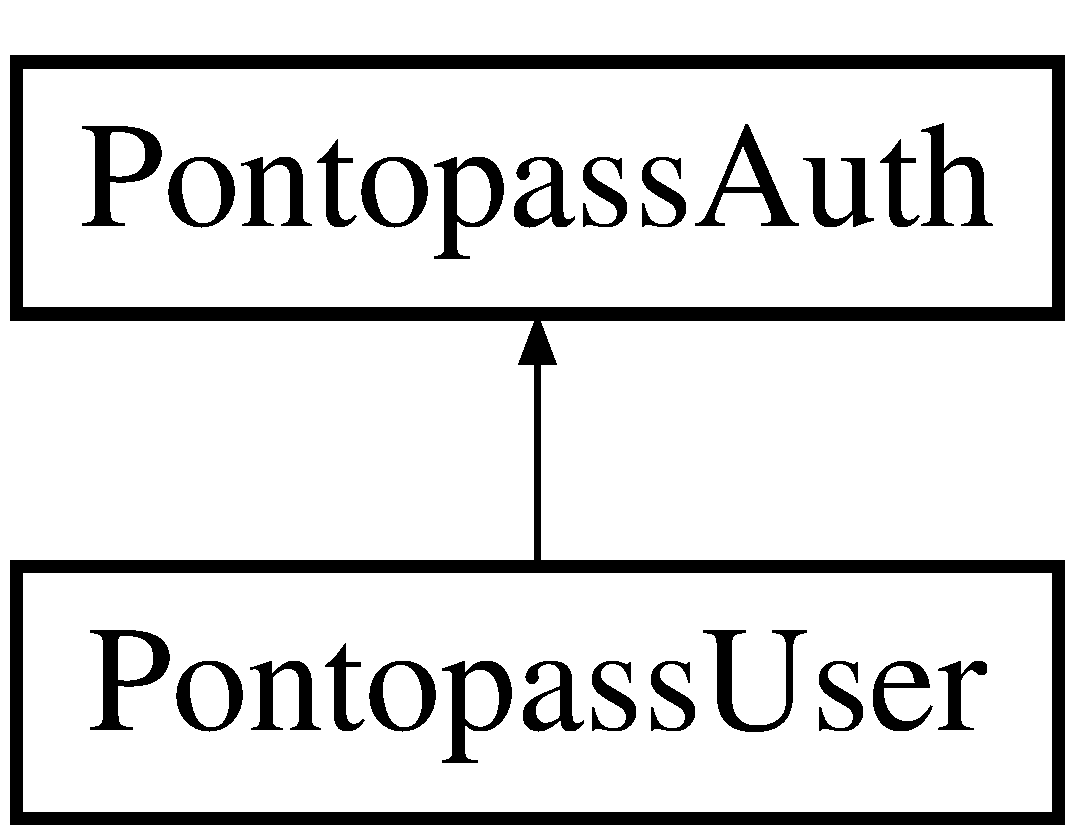
\includegraphics[height=2.000000cm]{classPontopassAuth}
\end{center}
\end{figure}
\subsection*{Membros públicos}
\begin{DoxyCompactItemize}
\item 
\hyperlink{classPontopassAuth_a5d0536d232e55faa0be69ff28548d5ea}{\-\_\-\-\_\-construct} (\$api\-\_\-id, \$api\-\_\-key, \$api\-\_\-server)
\item 
\hyperlink{classPontopassAuth_a12005841b570b001d21f6ec04bf2c42b}{last\-Status} ()
\item 
\hyperlink{classPontopassAuth_ad06637b1a81b1422fe0f7ade4b903609}{init} (\$username, \$use\-\_\-widget=T\-R\-U\-E, \$user\-\_\-remember=F\-A\-L\-S\-E, \$user\-\_\-ip=null, \$user\-\_\-agent=null)
\item 
\hyperlink{classPontopassAuth_af6e6a3a8fe54f83f5cc467a996edc830}{list\-Methods} ()
\item 
\hyperlink{classPontopassAuth_a7f65b17f3fca5e637db95d9675e96792}{ask} (\$device\-\_\-id)
\item 
\hyperlink{classPontopassAuth_ad4d35baf79f61ff2bdfc8f5767370745}{validate} (\$answer, \$token\-\_\-type)
\item 
\hyperlink{classPontopassAuth_a73eb1fb6dacf21f473f942f8e8eb5210}{widget} (\$h=500, \$w=500, \$return\-\_\-url, \$return\-\_\-method=\char`\"{}P\-O\-S\-T\char`\"{}, \$post=array(), \$get=array())
\item 
\hyperlink{classPontopassAuth_a8d1ea6eb1e30d8e9352d9bd750de1512}{check\-Answer} (\$username)
\item 
\hyperlink{classPontopassAuth_aeb5f569291b6923860bd31df480c8d6b}{status} ()
\end{DoxyCompactItemize}
\subsection*{Atributos Públicos}
\begin{DoxyCompactItemize}
\item 
\hypertarget{classPontopassAuth_a0a9de8521dadf8685bada54e995ad20f}{{\bfseries \$user\-\_\-agent}}\label{classPontopassAuth_a0a9de8521dadf8685bada54e995ad20f}

\item 
\hypertarget{classPontopassAuth_a8a71e97ba12b485685c568611d57c3c1}{{\bfseries \$user\-\_\-ip}}\label{classPontopassAuth_a8a71e97ba12b485685c568611d57c3c1}

\item 
\hypertarget{classPontopassAuth_acd34f947211dd0b266514ffb890d22cc}{{\bfseries \$user\-\_\-session}}\label{classPontopassAuth_acd34f947211dd0b266514ffb890d22cc}

\item 
\hypertarget{classPontopassAuth_a2f106279a0a3f00389172729c38031e1}{{\bfseries \$status}}\label{classPontopassAuth_a2f106279a0a3f00389172729c38031e1}

\end{DoxyCompactItemize}
\subsection*{Membros protegidos}
\begin{DoxyCompactItemize}
\item 
\hyperlink{classPontopassAuth_a85e61ad96f17e7c4fc9aec5d2124428b}{send} (\$path)
\end{DoxyCompactItemize}


\subsection{Descrição detalhada}
Copyright 2013 Pontosec Desenvolvimento e Solucoes em Tecnologia L\-T\-D\-A.

Licensed under the Apache License, Version 2.\-0 (the \char`\"{}\-License\char`\"{}); you may not use this file except in compliance with the License. You may obtain a copy of the License at \begin{DoxyVerb}http://www.apache.org/licenses/LICENSE-2.0
\end{DoxyVerb}


Unless required by applicable law or agreed to in writing, software distributed under the License is distributed on an \char`\"{}\-A\-S I\-S\char`\"{} B\-A\-S\-I\-S, W\-I\-T\-H\-O\-U\-T W\-A\-R\-R\-A\-N\-T\-I\-E\-S O\-R C\-O\-N\-D\-I\-T\-I\-O\-N\-S O\-F A\-N\-Y K\-I\-N\-D, either express or implied. See the License for the specific language governing permissions and limitations under the License.

Integracao com Web\-Service do Pontopass para confirmar a autenticacao de um usuario \begin{DoxyVersion}{Versão}
1.\-0 
\end{DoxyVersion}


\subsection{Documentação dos Construtores \& Destrutor}
\hypertarget{classPontopassAuth_a5d0536d232e55faa0be69ff28548d5ea}{\index{Pontopass\-Auth@{Pontopass\-Auth}!\-\_\-\-\_\-construct@{\-\_\-\-\_\-construct}}
\index{\-\_\-\-\_\-construct@{\-\_\-\-\_\-construct}!PontopassAuth@{Pontopass\-Auth}}
\subsubsection[{\-\_\-\-\_\-construct}]{\setlength{\rightskip}{0pt plus 5cm}Pontopass\-Auth\-::\-\_\-\-\_\-construct (
\begin{DoxyParamCaption}
\item[{}]{\$api\-\_\-id, }
\item[{}]{\$api\-\_\-key, }
\item[{}]{\$api\-\_\-server}
\end{DoxyParamCaption}
)}}\label{classPontopassAuth_a5d0536d232e55faa0be69ff28548d5ea}
Inicializacao;


\begin{DoxyParams}[1]{Parâmetros}
string & {\em \$api\-\_\-id} & I\-D de Integracao \\
\hline
string & {\em \$api\-\_\-key} & Chave de Integracao  public \\
\hline
\end{DoxyParams}


\subsection{Documentação dos métodos}
\hypertarget{classPontopassAuth_a7f65b17f3fca5e637db95d9675e96792}{\index{Pontopass\-Auth@{Pontopass\-Auth}!ask@{ask}}
\index{ask@{ask}!PontopassAuth@{Pontopass\-Auth}}
\subsubsection[{ask}]{\setlength{\rightskip}{0pt plus 5cm}Pontopass\-Auth\-::ask (
\begin{DoxyParamCaption}
\item[{}]{\$device\-\_\-id}
\end{DoxyParamCaption}
)}}\label{classPontopassAuth_a7f65b17f3fca5e637db95d9675e96792}
Solicita ao Pontopass que confirme a autenticacao do usuario utilizando determinado metodo


\begin{DoxyParams}[1]{Parâmetros}
int & {\em \$device\-\_\-id} & I\-D da forma de autenticacao a ser utilizada (obtida, por exemplo, pelo list\-Methods) \\
\hline
\end{DoxyParams}
\begin{DoxyReturn}{Retorna}
int Status Code retornado pelo Web\-Service  public 
\end{DoxyReturn}
\hypertarget{classPontopassAuth_a8d1ea6eb1e30d8e9352d9bd750de1512}{\index{Pontopass\-Auth@{Pontopass\-Auth}!check\-Answer@{check\-Answer}}
\index{check\-Answer@{check\-Answer}!PontopassAuth@{Pontopass\-Auth}}
\subsubsection[{check\-Answer}]{\setlength{\rightskip}{0pt plus 5cm}Pontopass\-Auth\-::check\-Answer (
\begin{DoxyParamCaption}
\item[{}]{\$username}
\end{DoxyParamCaption}
)}}\label{classPontopassAuth_a8d1ea6eb1e30d8e9352d9bd750de1512}
Verifica se a sessao de determinado usuario esta autenticada


\begin{DoxyParams}[1]{Parâmetros}
string & {\em \$username} & Nome do Usuario a ser verificado \\
\hline
\end{DoxyParams}
\begin{DoxyReturn}{Retorna}
bool T\-R\-U\-E para caso sessao esta autorizada, F\-A\-L\-S\-E para caso nao esteja autorizada  public 
\end{DoxyReturn}
\hypertarget{classPontopassAuth_ad06637b1a81b1422fe0f7ade4b903609}{\index{Pontopass\-Auth@{Pontopass\-Auth}!init@{init}}
\index{init@{init}!PontopassAuth@{Pontopass\-Auth}}
\subsubsection[{init}]{\setlength{\rightskip}{0pt plus 5cm}Pontopass\-Auth\-::init (
\begin{DoxyParamCaption}
\item[{}]{\$username, }
\item[{}]{\$use\-\_\-widget = {\ttfamily TRUE}, }
\item[{}]{\$user\-\_\-remember = {\ttfamily FALSE}, }
\item[{}]{\$user\-\_\-ip = {\ttfamily null}, }
\item[{}]{\$user\-\_\-agent = {\ttfamily null}}
\end{DoxyParamCaption}
)}}\label{classPontopassAuth_ad06637b1a81b1422fe0f7ade4b903609}
Inica sessao de autenticacao do Usuario


\begin{DoxyParams}[1]{Parâmetros}
string & {\em \$username} & Nome de usuario a ser autenticado \\
\hline
bool | null & {\em \$use\-\_\-widget} & T\-R\-U\-E para utilizar widget (frame) para os proximos passos da autenticacao, F\-A\-L\-S\-E para nao utilizar widget (frame) \\
\hline
bool | null & {\em \$user\-\_\-remember} & T\-R\-U\-E para gravar a sessao do usuario em cookie, F\-A\-L\-S\-E para nao gravar a sessao. \\
\hline
string | null & {\em \$user\-\_\-remember} & I\-P do Usuario (quando nao preenchido, obtido diretamente do request http) \\
\hline
string | null & {\em \$user\-\_\-agent} & User Agent do navegador do usuario (quando nao preenchido, obtido diretamente do request http) \\
\hline
\end{DoxyParams}
\begin{DoxyReturn}{Retorna}
int Status Code  public 
\end{DoxyReturn}
\hypertarget{classPontopassAuth_a12005841b570b001d21f6ec04bf2c42b}{\index{Pontopass\-Auth@{Pontopass\-Auth}!last\-Status@{last\-Status}}
\index{last\-Status@{last\-Status}!PontopassAuth@{Pontopass\-Auth}}
\subsubsection[{last\-Status}]{\setlength{\rightskip}{0pt plus 5cm}Pontopass\-Auth\-::last\-Status (
\begin{DoxyParamCaption}
{}
\end{DoxyParamCaption}
)}}\label{classPontopassAuth_a12005841b570b001d21f6ec04bf2c42b}
Retorna texto referente ao ultimo status respondido pelo Web\-Service

\begin{DoxyReturn}{Retorna}
string Mensagem do ultimo status respondido pelo Web\-Service  public 
\end{DoxyReturn}
\hypertarget{classPontopassAuth_af6e6a3a8fe54f83f5cc467a996edc830}{\index{Pontopass\-Auth@{Pontopass\-Auth}!list\-Methods@{list\-Methods}}
\index{list\-Methods@{list\-Methods}!PontopassAuth@{Pontopass\-Auth}}
\subsubsection[{list\-Methods}]{\setlength{\rightskip}{0pt plus 5cm}Pontopass\-Auth\-::list\-Methods (
\begin{DoxyParamCaption}
{}
\end{DoxyParamCaption}
)}}\label{classPontopassAuth_af6e6a3a8fe54f83f5cc467a996edc830}
Obtem todas as formas de confirmacao de login disponiveis para o usuario

\begin{DoxyReturn}{Retorna}
object Resposta do servidor (json decoded); F\-A\-L\-S\-E em caso de erros.  public 
\end{DoxyReturn}
\hypertarget{classPontopassAuth_a85e61ad96f17e7c4fc9aec5d2124428b}{\index{Pontopass\-Auth@{Pontopass\-Auth}!send@{send}}
\index{send@{send}!PontopassAuth@{Pontopass\-Auth}}
\subsubsection[{send}]{\setlength{\rightskip}{0pt plus 5cm}Pontopass\-Auth\-::send (
\begin{DoxyParamCaption}
\item[{}]{\$path}
\end{DoxyParamCaption}
)\hspace{0.3cm}{\ttfamily [protected]}}}\label{classPontopassAuth_a85e61ad96f17e7c4fc9aec5d2124428b}
Envia solicitacao ao Web\-Service


\begin{DoxyParams}[1]{Parâmetros}
string & {\em \$path} & Caminho a ser acessado \\
\hline
\end{DoxyParams}
\begin{DoxyReturn}{Retorna}
object Resposta do servidor (json decoded)  private 
\end{DoxyReturn}
\hypertarget{classPontopassAuth_aeb5f569291b6923860bd31df480c8d6b}{\index{Pontopass\-Auth@{Pontopass\-Auth}!status@{status}}
\index{status@{status}!PontopassAuth@{Pontopass\-Auth}}
\subsubsection[{status}]{\setlength{\rightskip}{0pt plus 5cm}Pontopass\-Auth\-::status (
\begin{DoxyParamCaption}
{}
\end{DoxyParamCaption}
)}}\label{classPontopassAuth_aeb5f569291b6923860bd31df480c8d6b}
Obtem ultimo Status Code da sessao no Web\-Service

\begin{DoxyReturn}{Retorna}
int Status Code da sessao  public 
\end{DoxyReturn}
\hypertarget{classPontopassAuth_ad4d35baf79f61ff2bdfc8f5767370745}{\index{Pontopass\-Auth@{Pontopass\-Auth}!validate@{validate}}
\index{validate@{validate}!PontopassAuth@{Pontopass\-Auth}}
\subsubsection[{validate}]{\setlength{\rightskip}{0pt plus 5cm}Pontopass\-Auth\-::validate (
\begin{DoxyParamCaption}
\item[{}]{\$answer, }
\item[{}]{\$token\-\_\-type}
\end{DoxyParamCaption}
)}}\label{classPontopassAuth_ad4d35baf79f61ff2bdfc8f5767370745}
Verifica codigo de confirmacao fornecido pelo usuario


\begin{DoxyParams}[1]{Parâmetros}
int & {\em \$answer} & Codigo de Confirmacao \\
\hline
int & {\em \$token\-\_\-type} & Codigo do tipo de confirmacao utilizado\-: 2 para S\-M\-S; 4 para Mobile Token \\
\hline
\end{DoxyParams}
\begin{DoxyReturn}{Retorna}
int Status Code retornado pelo Web\-Service  public 
\end{DoxyReturn}
\hypertarget{classPontopassAuth_a73eb1fb6dacf21f473f942f8e8eb5210}{\index{Pontopass\-Auth@{Pontopass\-Auth}!widget@{widget}}
\index{widget@{widget}!PontopassAuth@{Pontopass\-Auth}}
\subsubsection[{widget}]{\setlength{\rightskip}{0pt plus 5cm}Pontopass\-Auth\-::widget (
\begin{DoxyParamCaption}
\item[{}]{\$h = {\ttfamily 500}, }
\item[{}]{\$w = {\ttfamily 500}, }
\item[{}]{\$return\-\_\-url, }
\item[{}]{\$return\-\_\-method = {\ttfamily \char`\"{}POST\char`\"{}}, }
\item[{}]{\$post = {\ttfamily array()}, }
\item[{}]{\$get = {\ttfamily array()}}
\end{DoxyParamCaption}
)}}\label{classPontopassAuth_a73eb1fb6dacf21f473f942f8e8eb5210}
Gera codigo H\-T\-M\-L do iframe do widget de confirmacao.


\begin{DoxyParams}[1]{Parâmetros}
int | null & {\em \$h} & Altura do Iframe (default\-: 500) \\
\hline
int | null & {\em \$w} & Largura do Iframe (default\-: 500) \\
\hline
string & {\em \$return\-\_\-url} & U\-R\-L que recebe o retorno do Iframe \\
\hline
string | null & {\em \$return\-\_\-method} & Metodo H\-T\-T\-P para envio a U\-R\-L de Retorno. \char`\"{}\-P\-O\-S\-T\char`\"{} ou \char`\"{}\-G\-E\-T\char`\"{} (Default\-: P\-O\-S\-T) \\
\hline
array | null | null & {\em \$post} & Array contendo outros parametros que devem ser passados via P\-O\-S\-T para a U\-R\-L de Retorno \\
\hline
array | null & {\em \$get} & Array contendo outros parametros que devem ser passados via G\-E\-T para a U\-R\-L de Retorno \\
\hline
\end{DoxyParams}
\begin{DoxyReturn}{Retorna}
string Codigo H\-T\-M\-L do iframe do widget de confirmacao  public 
\end{DoxyReturn}


A documentação para esta classe foi gerada a partir do seguinte ficheiro\-:\begin{DoxyCompactItemize}
\item 
pontopass\-\_\-sdk.\-php\end{DoxyCompactItemize}

\hypertarget{classPontopassUser}{\section{Referência à classe Pontopass\-User}
\label{classPontopassUser}\index{Pontopass\-User@{Pontopass\-User}}
}
Diagrama de heranças da classe Pontopass\-User\begin{figure}[H]
\begin{center}
\leavevmode
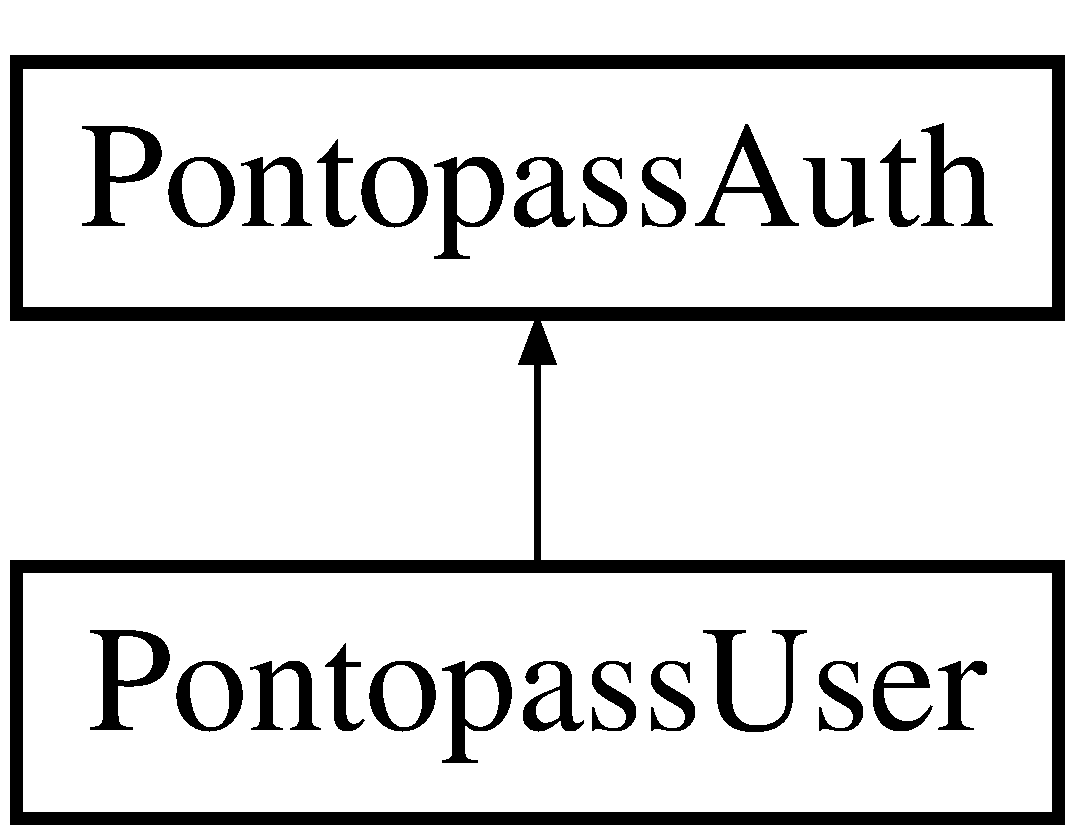
\includegraphics[height=2.000000cm]{classPontopassUser}
\end{center}
\end{figure}
\subsection*{Membros públicos}
\begin{DoxyCompactItemize}
\item 
\hyperlink{classPontopassUser_ac357568a924218947ad8d56608ebd54a}{create} (\$name=\char`\"{}\char`\"{})
\item 
\hyperlink{classPontopassUser_aa07fc177a4efec331e7919ad847b2a02}{delete} ()
\item 
\hyperlink{classPontopassUser_afae4d293eefebe500c3f6937755cb1db}{insert\-Device} (\$type, \$phone, \$desc=null)
\item 
\hyperlink{classPontopassUser_aa801f31c2272a106c99cae5e8d95560e}{delete\-Device} (\$methodid)
\item 
\hyperlink{classPontopassUser_a354d501dc79433784c236dbf46c6641a}{check\-Method} (\$methodid)
\item 
\hyperlink{classPontopassUser_a054a98aa1525a632f5ccffe3d2776e72}{exists} ()
\item 
\hyperlink{classPontopassUser_af9b7615674b739effeff9c9eca361939}{list\-Methods} ()
\end{DoxyCompactItemize}
\subsection*{Atributos Públicos}
\begin{DoxyCompactItemize}
\item 
\hypertarget{classPontopassUser_a396a17b0b901b42078dd38c5fecde6e6}{{\bfseries \$login}}\label{classPontopassUser_a396a17b0b901b42078dd38c5fecde6e6}

\end{DoxyCompactItemize}
\subsection*{Additional Inherited Members}


\subsection{Descrição detalhada}
Auxilia o gerenciamento de usuarios e dispositivos cadastrados na base do Pontopass \begin{DoxyVersion}{Versão}
1.\-0 
\end{DoxyVersion}


\subsection{Documentação dos métodos}
\hypertarget{classPontopassUser_a354d501dc79433784c236dbf46c6641a}{\index{Pontopass\-User@{Pontopass\-User}!check\-Method@{check\-Method}}
\index{check\-Method@{check\-Method}!PontopassUser@{Pontopass\-User}}
\subsubsection[{check\-Method}]{\setlength{\rightskip}{0pt plus 5cm}Pontopass\-User\-::check\-Method (
\begin{DoxyParamCaption}
\item[{}]{\$methodid}
\end{DoxyParamCaption}
)}}\label{classPontopassUser_a354d501dc79433784c236dbf46c6641a}
Verifica se determinado dispositivo (methodid) pertence a um usuario


\begin{DoxyParams}[1]{Parâmetros}
int & {\em \$methodid} & I\-D do dispositivo a ser verificado \\
\hline
\end{DoxyParams}
\begin{DoxyReturn}{Retorna}
int Status Code da operacao retornado pelo Web\-Service  public 
\end{DoxyReturn}
\hypertarget{classPontopassUser_ac357568a924218947ad8d56608ebd54a}{\index{Pontopass\-User@{Pontopass\-User}!create@{create}}
\index{create@{create}!PontopassUser@{Pontopass\-User}}
\subsubsection[{create}]{\setlength{\rightskip}{0pt plus 5cm}Pontopass\-User\-::create (
\begin{DoxyParamCaption}
\item[{}]{\$name = {\ttfamily \char`\"{}\char`\"{}}}
\end{DoxyParamCaption}
)}}\label{classPontopassUser_ac357568a924218947ad8d56608ebd54a}
Cadastra novo usuario


\begin{DoxyParams}[1]{Parâmetros}
string | null & {\em \$name} & Nome do Usuario (ou outra informacao para identifica-\/lo) -\/ Opcional \\
\hline
\end{DoxyParams}
\begin{DoxyReturn}{Retorna}
int Status Code da operacao retornado pelo Web\-Service  public 
\end{DoxyReturn}
\hypertarget{classPontopassUser_aa07fc177a4efec331e7919ad847b2a02}{\index{Pontopass\-User@{Pontopass\-User}!delete@{delete}}
\index{delete@{delete}!PontopassUser@{Pontopass\-User}}
\subsubsection[{delete}]{\setlength{\rightskip}{0pt plus 5cm}Pontopass\-User\-::delete (
\begin{DoxyParamCaption}
{}
\end{DoxyParamCaption}
)}}\label{classPontopassUser_aa07fc177a4efec331e7919ad847b2a02}
Deleta Usuario

\begin{DoxyReturn}{Retorna}
int Status Code da operacao retornado pelo Web\-Service  public 
\end{DoxyReturn}
\hypertarget{classPontopassUser_aa801f31c2272a106c99cae5e8d95560e}{\index{Pontopass\-User@{Pontopass\-User}!delete\-Device@{delete\-Device}}
\index{delete\-Device@{delete\-Device}!PontopassUser@{Pontopass\-User}}
\subsubsection[{delete\-Device}]{\setlength{\rightskip}{0pt plus 5cm}Pontopass\-User\-::delete\-Device (
\begin{DoxyParamCaption}
\item[{}]{\$methodid}
\end{DoxyParamCaption}
)}}\label{classPontopassUser_aa801f31c2272a106c99cae5e8d95560e}
Cadastra dispositivo do usuario


\begin{DoxyParams}[1]{Parâmetros}
int & {\em \$methodid} & I\-D do dispositivo a ser removido \\
\hline
\end{DoxyParams}
\begin{DoxyReturn}{Retorna}
int Status Code da operacao retornado pelo Web\-Service  public 
\end{DoxyReturn}
\hypertarget{classPontopassUser_a054a98aa1525a632f5ccffe3d2776e72}{\index{Pontopass\-User@{Pontopass\-User}!exists@{exists}}
\index{exists@{exists}!PontopassUser@{Pontopass\-User}}
\subsubsection[{exists}]{\setlength{\rightskip}{0pt plus 5cm}Pontopass\-User\-::exists (
\begin{DoxyParamCaption}
{}
\end{DoxyParamCaption}
)}}\label{classPontopassUser_a054a98aa1525a632f5ccffe3d2776e72}
Verifica se determinado login esta cadastrado na base de usuarios do Pontopass


\begin{DoxyParams}[1]{Parâmetros}
int & {\em \$methodid} & I\-D do dispositivo a ser verificado \\
\hline
\end{DoxyParams}
\begin{DoxyReturn}{Retorna}
int Status Code da operacao retornado pelo Web\-Service  public 
\end{DoxyReturn}
\hypertarget{classPontopassUser_afae4d293eefebe500c3f6937755cb1db}{\index{Pontopass\-User@{Pontopass\-User}!insert\-Device@{insert\-Device}}
\index{insert\-Device@{insert\-Device}!PontopassUser@{Pontopass\-User}}
\subsubsection[{insert\-Device}]{\setlength{\rightskip}{0pt plus 5cm}Pontopass\-User\-::insert\-Device (
\begin{DoxyParamCaption}
\item[{}]{\$type, }
\item[{}]{\$phone, }
\item[{}]{\$desc = {\ttfamily null}}
\end{DoxyParamCaption}
)}}\label{classPontopassUser_afae4d293eefebe500c3f6937755cb1db}
Cadastra dispositivo do usuario


\begin{DoxyParams}[1]{Parâmetros}
int & {\em \$type} & Forma de Autenticacao a ser utilizada (1 para ligacao telefonica, 2 para codigo por sms, 3 para confirmacao por app mobile, 4 por codigo de mobile token) \\
\hline
string & {\em \$phone} & Telefone do Usuario, incluindo codigo do pais e da cidade, sem 0 de prefixo, sem + de prefixo. \\
\hline
string | null & {\em \$desc} & Descricao do Dispositivo (ex\-: Celular do Roberto) -\/ Opcional \\
\hline
\end{DoxyParams}
\begin{DoxyReturn}{Retorna}
int Status Code da operacao retornado pelo Web\-Service  public 
\end{DoxyReturn}
\hypertarget{classPontopassUser_af9b7615674b739effeff9c9eca361939}{\index{Pontopass\-User@{Pontopass\-User}!list\-Methods@{list\-Methods}}
\index{list\-Methods@{list\-Methods}!PontopassUser@{Pontopass\-User}}
\subsubsection[{list\-Methods}]{\setlength{\rightskip}{0pt plus 5cm}Pontopass\-User\-::list\-Methods (
\begin{DoxyParamCaption}
{}
\end{DoxyParamCaption}
)}}\label{classPontopassUser_af9b7615674b739effeff9c9eca361939}
Lista dispositivos de um usuario

\begin{DoxyReturn}{Retorna}
object Relacao de Dispositivos do Usuario  public 
\end{DoxyReturn}


A documentação para esta classe foi gerada a partir do seguinte ficheiro\-:\begin{DoxyCompactItemize}
\item 
pontopass\-\_\-sdk.\-php\end{DoxyCompactItemize}

%--- End generated contents ---

% Index
\newpage
\phantomsection
\addcontentsline{toc}{part}{Índice}
\printindex

\end{document}
